\documentclass{article}

\usepackage{graphicx}
\usepackage{tikz}
\usepackage{tikzsymbols}
\usetikzlibrary{calc,patterns,shapes.geometric}
\pagestyle{empty}
\usepackage[margin=0pt]{geometry}
\geometry{papersize={14in,12in}}

\def\centerarc[#1](#2)(#3:#4:#5){\draw[#1] ($(#2)+({#5*cos(#3)},{#5*sin(#3)})$) arc (#3:#4:#5);}

\begin{document}
	\begin{figure}
		\centering
		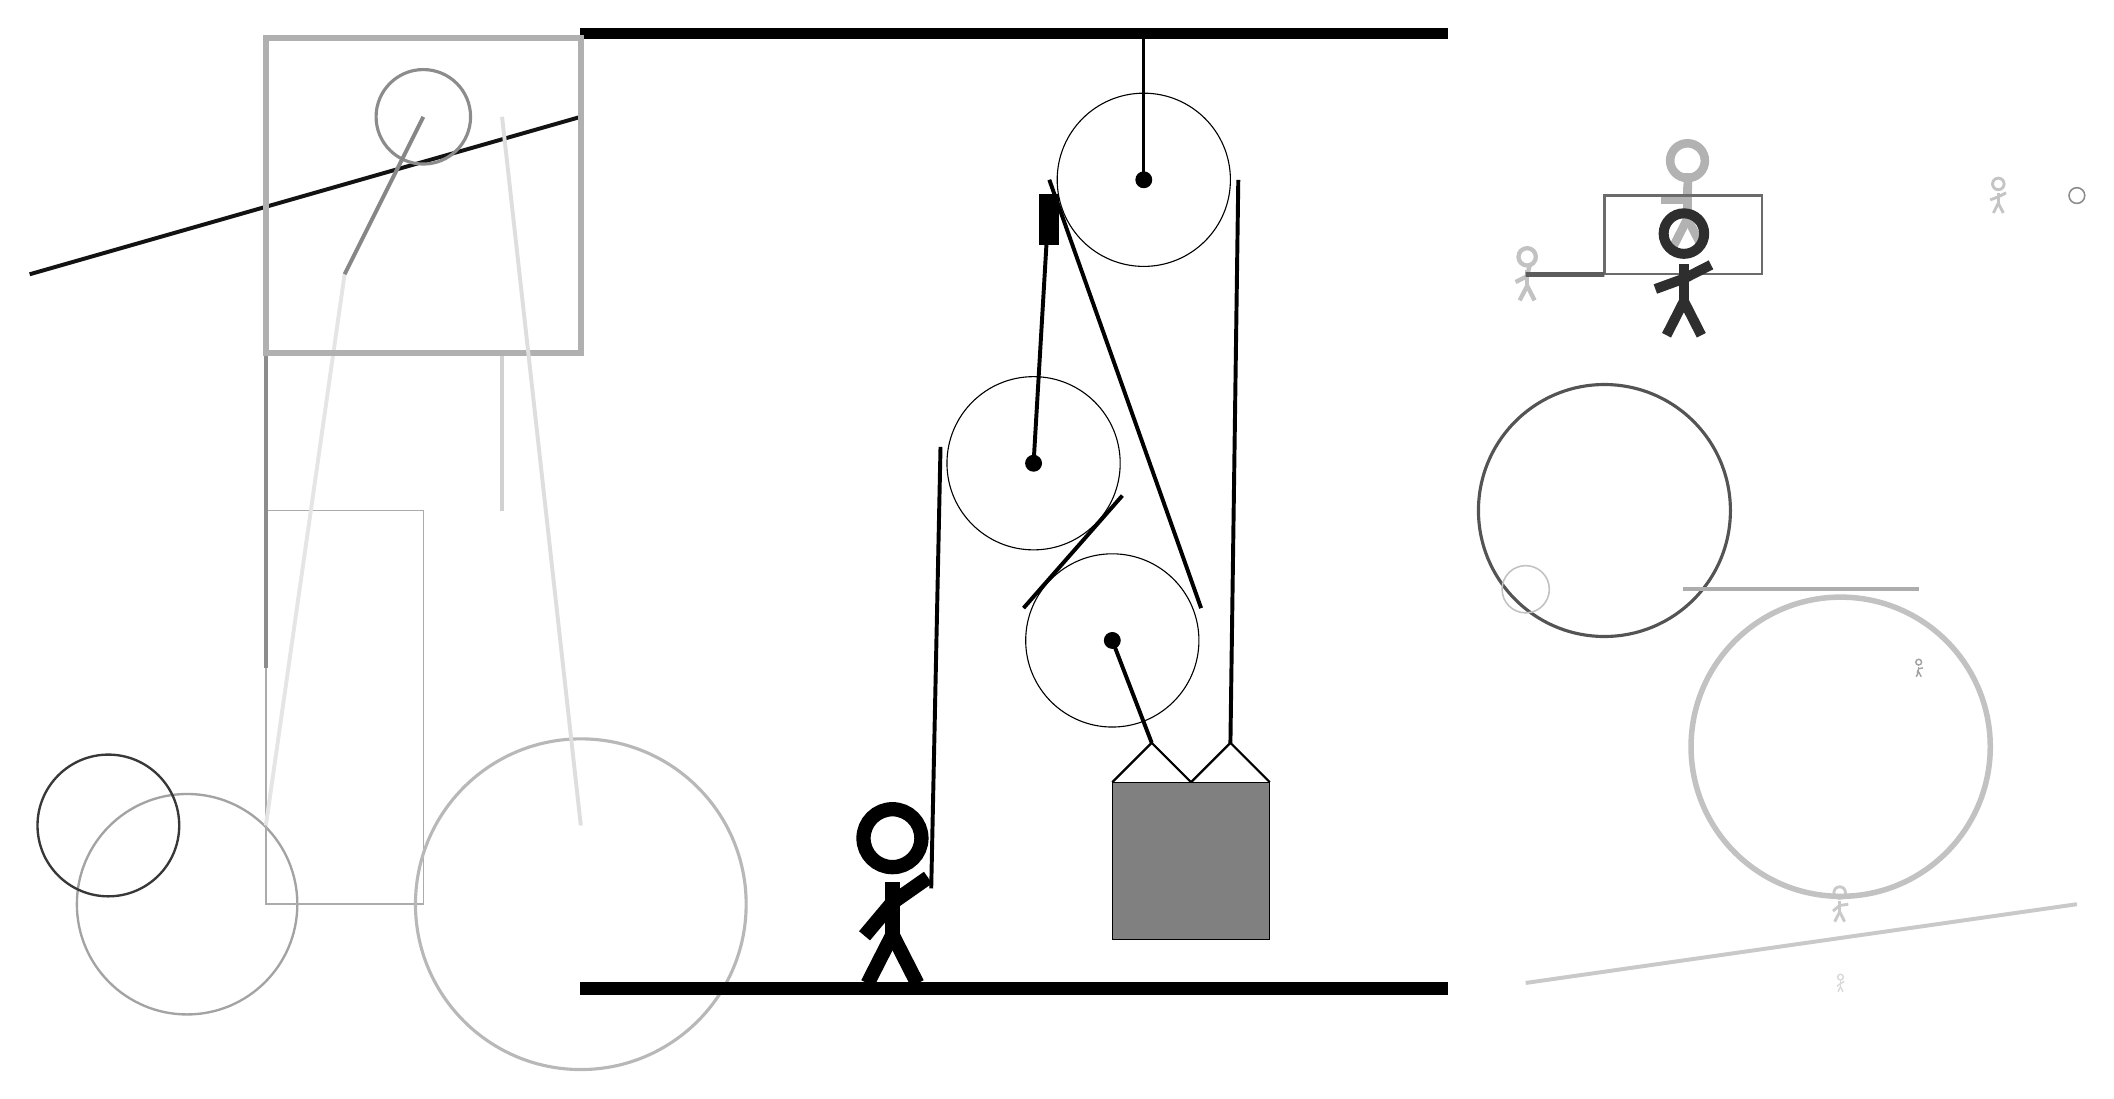
\begin{tikzpicture}
			%%%%% START %%%%%
			
			\draw[fill=black] (-6, 9) rectangle (5, 9.125);
			
			\draw (-0.25, 3.6) circle (1.1);
			\draw[fill=black] (-0.25, 3.6) circle (0.1);
			
			\draw (0.75, 1.35) circle (1.1);
			\draw[fill=black] (0.75, 1.35) circle (0.1);
			
			\draw (1.15, 7.2) circle (1.1);
			\draw[fill=black] (1.15, 7.2) circle (0.1);
			\draw[very thick] (1.15, 7.2) -- (1.15, 9);
			
			\draw [line width=0.3mm, color=black!36](-11, -2) circle (1.4);
			
			\node[line width=0.7mm, color=black!24] at (6, 6) {\Strichmaxerl[3][27][77]};
			\draw [line width=0.4mm, color=black!67](7, 3) circle (1.6);
			\node[line width=0.6mm, color=black!30] at (8, 7) {\Strichmaxerl[6][0][89]};
			\draw[line width=0.3mm, color=black!58] (7, 6) rectangle (9, 7);
			\node[line width=0.7mm, color=black!37] at (11, 1) {\Strichmaxerl[1][70][9]};
			\draw[line width=0.2mm, color=black!33] (-8, 3) rectangle (-10, -2);
			\draw[line width=0.5mm, color=black!32](8, 2) -- (11, 2);
			\node[line width=0.5mm, color=black!15] at (10, -3) {\Strichmaxerl[1][38][31]};
			
			\node[line width=0.5mm, color=black!82] at (8, 6) {\Strichmaxerl[7][20][27]};
			\draw [line width=0.4mm, color=black!28](-6, -2) circle (2.1);
			\node[line width=0.4mm, color=black!21] at (10, -2) {\Strichmaxerl[2][40][8]};
			\draw[line width=0.5mm, color=black!93](-6, 8) -- (-13, 6);
			
			\draw [line width=0.7mm, color=black!24](10, 0) circle (1.9);
			\draw[line width=0.5mm, color=black!10](-10, -1) -- (-9, 6);
			\draw [line width=0.4mm, color=black!45](-8, 8) circle (0.6);
			\draw[line width=0.5mm, color=black!45](-10, 1) -- (-10, 9);
			\draw[line width=0.5mm, color=black!18](-7, 3) -- (-7, 5);
			\draw [line width=0.2mm, color=black!24](6, 2) circle (0.3);
			\draw[line width=0.7mm, color=black!31] (-6, 5) rectangle (-10, 9);
			\draw[line width=0.6mm, color=black!64] (7, 6) rectangle (6, 6);
			
			\node[line width=0.4mm, color=black!23] at (12, 7) {\Strichmaxerl[2][21][27]};
			
			\draw[line width=0.5mm, color=black!47](-8, 8) -- (-9, 6);
			\draw [line width=0.2mm, color=black!45](13, 7) circle (0.1);
			\draw[line width=0.5mm, color=black!21](6, -3) -- (13, -2);
			
			\draw [line width=0.3mm, color=black!78](-12, -1) circle (0.9);
			\draw[line width=0.5mm, color=black!13](-7, 8) -- (-6, -1);
			
			\draw[thick]  (0.75, -0.45) -- (1.25, 0.05) -- (1.75, -0.45) -- (2.25, 0.05) -- (2.75, -0.45);
			\draw[fill=black!50] (0.75, -0.45) rectangle (2.75, -2.45);
			
			\draw[line width=0.5mm] (-0.25, 3.6) -- (-0.05, 7.0);
			\draw[line width=0.5mm, fill=black](-0.15, 6.4) rectangle (0.05, 7.0);
			\draw[line width=0.5mm] (-1.55, -1.8) -- (-1.4318, 3.8083);
			\centerarc[line width=0.5mm](-0.25, 3.6)(-20:170:1.2000000000000002);
			\draw[line width=0.5mm] (0.8776, 3.1896) -- (-0.3776, 1.7604);
			\centerarc[line width=0.5mm](0.75, 1.35)(160:380:1.2000000000000002);
			\draw[line width=0.5mm] (1.8776, 1.7604) -- (-0.05, 7.2);
			\draw[line width=0.5mm](0.75, 1.35) -- (1.25, 0.05);
			\centerarc[line width=0.5mm](1.15, 7.2)(0:180:1.2000000000000002);
			\draw[line width=0.5mm] (2.35, 7.2) -- (2.25, 0.05);
			
			\node at (-2, -1.9) {\Strichmaxerl[10][50][35]};
			
			\draw[fill=black] (-6, -3) rectangle (5, -3.15);
			
			%%%%% END %%%%%
		\end{tikzpicture}
	\end{figure}	
\end{document}